%%%%%%%%%%%%%%%%%%%%%%%%%%%%%%%%%%%%%%%%%
% KOMA-Script Presentation
% LaTeX Template
% Version 1.1 (18/10/15)
%
% This template has been downloaded from:
% http://www.LaTeXTemplates.com
%
% Original Authors:
% Marius Hofert (marius.hofert@math.ethz.ch)
% Markus Kohm (komascript@gmx.info)
% Described in the PracTeX Journal, 2010, No. 2
%
% License:
% CC BY-NC-SA 3.0 (http://creativecommons.org/licenses/by-nc-sa/3.0/)
%
%%%%%%%%%%%%%%%%%%%%%%%%%%%%%%%%%%%%%%%%%

%----------------------------------------------------------------------------------------
%	PACKAGES AND OTHER DOCUMENT CONFIGURATIONS
%----------------------------------------------------------------------------------------

\documentclass[
paper=128mm:96mm, % The same paper size as used in the beamer class
fontsize=11pt, % Font size
pagesize, % Write page size to dvi or pdf
parskip=half-, % Paragraphs separated by half a line
]{scrartcl} % KOMA script (article)

\linespread{1.12} % Increase line spacing for readability

%------------------------------------------------
% Colors
\usepackage[dvipsnames]{xcolor}	 % Required for custom colors
% Define a few colors for making text stand out within the presentation
\definecolor{mygreen}{RGB}{44,85,17}
\definecolor{myblue}{RGB}{34,31,217}
\definecolor{mybrown}{RGB}{194,164,113}
\definecolor{myred}{RGB}{255,66,56}
% Use these colors within the presentation by enclosing text in the commands below
\newcommand*{\mygreen}[1]{\textcolor{mygreen}{#1}}
\newcommand*{\myblue}[1]{\textcolor{myblue}{#1}}
\newcommand*{\mybrown}[1]{\textcolor{mybrown}{#1}}
\newcommand*{\myred}[1]{\textcolor{myred}{#1}}
%------------------------------------------------

%------------------------------------------------
% Margins
\usepackage[ % Page margins settings
includeheadfoot,
top=3.5mm,
bottom=3.5mm,
left=5.5mm,
right=5.5mm,
headsep=6.5mm,
footskip=8.5mm
]{geometry}
%------------------------------------------------

%------------------------------------------------
% Fonts
\usepackage[T1]{fontenc}	 % For correct hyphenation and T1 encoding
\usepackage{lmodern} % Default font: latin modern font
%\usepackage{fourier} % Alternative font: utopia
%\usepackage{charter} % Alternative font: low-resolution roman font
\renewcommand{\familydefault}{\sfdefault} % Sans serif - this may need to be commented to see the alternative fonts
%------------------------------------------------

%------------------------------------------------
% Various required packages
\usepackage{amsthm} % Required for theorem environments
\usepackage{bm} % Required for bold math symbols (used in the footer of the slides)
\usepackage{graphicx} % Required for including images in figures
\usepackage{tikz} % Required for colored boxes
\usepackage{booktabs} % Required for horizontal rules in tables
\usepackage{multicol} % Required for creating multiple columns in slides
\usepackage{lastpage} % For printing the total number of pages at the bottom of each slide
\usepackage[english]{babel} % Document language - required for customizing section titles
\usepackage{microtype} % Better typography
\usepackage{tocstyle} % Required for customizing the table of contents
%------------------------------------------------

%------------------------------------------------
% Slide layout configuration
\usepackage{scrpage2} % Required for customization of the header and footer
\pagestyle{scrheadings} % Activates the pagestyle from scrpage2 for custom headers and footers
\clearscrheadfoot % Remove the default header and footer
\setkomafont{pageheadfoot}{\normalfont\color{black}\sffamily} % Font settings for the header and footer

% Sets vertical centering of slide contents with increased space between paragraphs/lists
\makeatletter
\renewcommand*{\@textbottom}{\vskip \z@ \@plus 1fil}
\newcommand*{\@texttop}{\vskip \z@ \@plus .5fil}
\addtolength{\parskip}{\z@\@plus .25fil}
\makeatother

% Remove page numbers and the dots leading to them from the outline slide
\makeatletter
\newtocstyle[noonewithdot]{nodotnopagenumber}{\settocfeature{pagenumberbox}{\@gobble}}
\makeatother
\usetocstyle{nodotnopagenumber}

\AtBeginDocument{\renewcaptionname{english}{\contentsname}{\Large Math Time}} % Change the name of the table of contents
%------------------------------------------------

%------------------------------------------------
% Header configuration - if you don't want a header remove this block
\ihead{
\hspace{-2mm}
\begin{tikzpicture}[remember picture,overlay]
\node [xshift=\paperwidth/2,yshift=-\headheight] (mybar) at (current page.north west)[rectangle,fill,inner sep=0pt,minimum width=\paperwidth,minimum height=2\headheight,top color=mygreen!64,bottom color=mygreen]{}; % Colored bar
\node[below of=mybar,yshift=3.3mm,rectangle,shade,inner sep=0pt,minimum width=128mm,minimum height =1.5mm,top color=black!50,bottom color=white]{}; % Shadow under the colored bar
shadow
\end{tikzpicture}
\color{white}\runninghead} % Header text defined by the \runninghead command below and colored white for contrast
%------------------------------------------------

%------------------------------------------------
% Footer configuration
\setlength{\footheight}{8mm} % Height of the footer
\addtokomafont{pagefoot}{\footnotesize} % Small font size for the footnote

\ifoot{% Left side
\hspace{-2mm}
\begin{tikzpicture}[remember picture,overlay]
\node [xshift=\paperwidth/2,yshift=\footheight] at (current page.south west)[rectangle,fill,inner sep=0pt,minimum width=\paperwidth,minimum height=3pt,top color=mygreen,bottom color=mygreen]{}; % Green bar
\end{tikzpicture}
\myauthor\ \raisebox{0.2mm}{$\bm{\vert}$}\ \myuni % Left side text
}

\ofoot[\pagemark/\pageref{LastPage}\hspace{-2mm}]{\pagemark/\pageref{LastPage}\hspace{-2mm}} % Right side
%------------------------------------------------

%------------------------------------------------
% Section spacing - deeper section titles are given less space due to lesser importance
%\usepackage{titlesec} % Required for customizing section spacing
%\titlespacing{\section}{1mm}{1mm}{1mm} % Lengths are: left, before, after
%\titlespacing{\subsection}{0mm}{0mm}{-1mm} % Lengths are: left, before, after
%\titlespacing{\subsubsection}{0mm}{0mm}{-2mm} % Lengths are: left, before, after
%\setcounter{secnumdepth}{0} % How deep sections are numbered, set to no numbering by default - change to 1 for numbering sections, 2 for numbering sections and subsections, etc
%------------------------------------------------

%------------------------------------------------
% Theorem style
\newtheoremstyle{mythmstyle} % Defines a new theorem style used in this template
{0.5em} % Space above
{0.5em} % Space below
{} % Body font
{} % Indent amount
{\sffamily\bfseries} % Head font
{} % Punctuation after head
{\newline} % Space after head
{\thmname{#1}\ \thmnote{(#3)}} % Head spec
	
\theoremstyle{mythmstyle} % Change the default style of the theorem to the one defined above
\newtheorem{theorem}{Theorem}[section] % Label for theorems
\newtheorem{prob}{Problem}[section]  %Label for problems 
\newtheorem{lemma}{Lemma}[section]  %Label for lemmas 
\newtheorem{defi}{Definition}[section]
\newtheorem{exmp}{Exercise}[section] %Label for examples
\newtheorem{remark}[theorem]{Remark} % Label for remarks
\newtheorem{algorithm}[theorem]{Algorithm} % Label for algorithms
\makeatletter % Correct qed adjustment
%------------------------------------------------

%------------------------------------------------
% The code for the box which can be used to highlight an element of a slide (such as a theorem)
\newcommand*{\mybox}[2]{ % The box takes two arguments: width and content
\par\noindent
\begin{tikzpicture}[mynodestyle/.style={rectangle,draw=mygreen,thick,inner sep=2mm,text justified,top color=white,bottom color=white,above}]\node[mynodestyle,at={(0.5*#1+2mm+0.4pt,0)}]{ % Box formatting
\begin{minipage}[t]{#1}
#2
\end{minipage}
};
\end{tikzpicture}
\par\vspace{-1.3em}}
%------------------------------------------------

%------------------------------------------------
% MODIFICATIONS BY JUSTIN STEVENS
%------------------------------------------------

\usepackage[nodayofweek,level]{datetime}
\usepackage{caption}
\usepackage{subcaption}
\usepackage{hyperref}
\newcommand{\pmid}{\mid\!\mid}
\usepackage{seqsplit}
\usepackage{amsfonts}
\usepackage{float} %use H to force it in place
\usepackage{amssymb} %for nmid
\usepackage{enumitem} %for itemized lists with stars
\usepackage{amsmath}
\DeclareMathOperator{\lcm}{lcm}
%\usepackage{epigraph}
\usepackage{csquotes}
\usepackage{relsize}
\newcommand{\x}{\color{red}X\color{black}}




%----------------------------------------------------------------------------------------
%	PRESENTATION INFORMATION
%----------------------------------------------------------------------------------------

\newcommand*{\mytitle}{A-Star 2016 Winter Math Camp } % Title
\newcommand*{\runninghead}{AMC Algebra} % Running head displayed on almost all slides
\newcommand*{\myauthor}{Justin Stevens} % Presenters name(s)
\newcommand*{\mydate}{\formatdate{26}{12}{2016}} % Presentation date
\newcommand*{\myuni}{A-Star 2016 Winter Math Camp} % University or department

%----------------------------------------------------------------------------------------

\begin{document}
	

%----------------------------------------------------------------------------------------
%	TITLE SLIDE
%----------------------------------------------------------------------------------------

% Title slide - you may have to tweak a few of the numbers if you wish to make changes to the layout
\thispagestyle{empty} % No slide header and footer
\begin{tikzpicture}[remember picture,overlay] % Background box
\node [xshift=\paperwidth/2,yshift=\paperheight/2] at (current page.south west)[rectangle,fill,inner sep=0pt,minimum width=\paperwidth,minimum height=\paperheight/3,top color=mygreen,bottom color=mygreen]{}; % Change the height of the box, its colors and position on the page here
\end{tikzpicture}
% Text within the box
\begin{flushright}
\vspace{0.6cm}
\color{white}\sffamily
{\bfseries\Large\mytitle\par} % Title
\vspace{0.5cm}
\normalsize
\myauthor\par % Author name
\mydate\par % Date
\vfill
\end{flushright}



\clearpage


%----------------------------------------------------------------------------------------
%	TABLE OF CONTENTS
%----------------------------------------------------------------------------------------

\thispagestyle{empty} % No slide header and footer

\small\tableofcontents % Change the font size and print the table of contents - it may be useful to shrink the font size further if the presentation is full of sections
% To exclude sections/subsections from the table of contents, put an asterisk after \(sub)section like so: \section*{Section Name}

\clearpage

\section{Algebraic Manipulation}


\begin{figure}[H]
	\centering\includegraphics[width=0.7\linewidth]{images/joke.jpg}
\end{figure}

\mybox{0.8\textwidth}{\begin{prob}[2000 AMC 12]  If $x,y,$ and $z$ are positive numbers satisfying $$x+\frac{1}{y}=4\:, y+\frac{1}{z}=1\:, \text{and}\: z+\frac{1}{x}=\frac73,$$ find the value of $xyz$. \end{prob} \begin{prob}[AoPS Introduction to Algebra] Let $A=x+\frac{1}{x}$ and $B=x^2+\frac{1}{x^2}$. Note that $(x+\frac{1}{x})^2=x^2+2+\frac{1}{x^2}$, therefore, $B=A^2-2$. Find formulas for $$C=x^3+\frac{1}{x^3}\:, D=x^4+\frac{1}{x^4}, E=x^5+\frac{1}{x^5}$$ in terms of $A$.  \end{prob}}

\subsection{2000 AMC 12}
\begin{proof}[Solution]
In order to get the $xyz$ term, we are motivated to multiply the $3$ equations together: \begin{eqnarray*} \left(x+\frac{1}{y}\right)\left(y+\frac{1}{z}\right)\left(z+\frac{1}{x}\right)&=&xyz+\frac{1}{xyz}+\left(x+y+z\right)+\left(\frac{1}{x}+\frac{1}{y}+\frac{1}{z}\right) \\ &=& \left(4\right)\left(1\right)\left(\frac73\right)=\frac{28}{3}. \end{eqnarray*}  

What can we do now to simplify this further?
\clearpage
We also add all $3$ of the equations: \begin{eqnarray*} \left(x+\frac{1}{y}\right)+\left(y+\frac{1}{z}\right)+\left(z+\frac{1}{x}\right)&=&4+1+\frac{7}{3}=\frac{22}{3} \\ &=& \left(x+y+z\right)+\left(\frac{1}{x}+\frac{1}{y}+\frac{1}{z}\right). \end{eqnarray*}  
Therefore, plugging this in to the first equation gives \begin{eqnarray*} xyz+\frac{1}{xyz}+\left(x+y+z\right)+\left(\frac{1}{x}+\frac{1}{y}+\frac{1}{z}\right) &=& xyz+\frac{1}{xyz}+\frac{22}{3} \\ &=&\frac{28}{3} \\ \implies \color{blue} xyz+\frac{1}{xyz} &=& \color{blue} 2. \end{eqnarray*}  

What's $xyz$ equal to then?

\clearpage

Multiply the equation through by $xyz$ and simplify: $$(xyz)^2+1=2xyz\implies (xyz)^2-2\cdot xyz+1=(xyz-1)^2=0.$$  
Therefore, $xyz=\boxed{1}$.  \end{proof}

\subsection{Exponent Mayhem} 

\begin{proof}[Solution]
	
We begin with $C$. Inspired by our method for computing $B$, we attempt to cube $x+\frac{1}{x}$: \begin{eqnarray*} (x+\frac{1}{x})^3&=&x^3+3\cdot x^2\cdot \frac{1}{x}+3\cdot x\cdot \frac{1}{x^2}+\frac{1}{x^3} \\ &=& x^3+3x+\frac{3}{x}+\frac{1}{x^3}. \end{eqnarray*} 
\clearpage

Therefore, \begin{eqnarray*} A^3&=&x^3+3\left(x+\frac{1}{x}\right)+\frac{1}{x^3} \:=\:C+3A \\ \implies \color{blue} C &=& \color{blue} A^3-3A. \end{eqnarray*}

There are two methods for finding $D$. One of them involves taking $x+\frac{1}{x}$ to the fourth power. In order to continue with this method, however, I must introduce the binomial theorem and Pascal's triangle.  

\clearpage
\subsection{Pascal's Triangle}

\begin{figure}[h]
	\centering\includegraphics[width=0.36\linewidth]{images/pascal.jpg}
	\caption{Source:  iCoachMath.com}
\end{figure}

\clearpage

\subsection{Binomial-theorem}
The binomial theorem states that when we expand $x+y$ to the $n$th power, the coefficients will be the numbers in the $n$th row of Pascal's triangle. For instance, $$(x+y)^4=\textbf{1}x^4+\textbf{4}x^3y+\textbf{6}x^2y^2+\textbf{4}xy^3+\textbf{1}y^4.$$
The numbers $1, 4, 6, 4, 1$ make up the $4$th row of Pascal's triangle. Furthermore, if you know binomial coefficients, note that $$\binom{4}{0}=1, \binom{4}{1}=4, \binom{4}{2}=6, \binom{4}{3}=4, \binom{4}{4}=1.$$

\mybox{0.8\textwidth}{\begin{theorem}[Binomial Expansion] $$(x+y)^n=\displaystyle \sum_{k=0}^{n}\binom{n}{k}x^ky^{n-k}.$$ \end{theorem}}

Using the expansion for $(x+y)^4$, we see that \begin{eqnarray*} (x+\frac{1}{x})^4&=&x^4+4\cdot \left(x^3\cdot \frac{1}{x}\right)+6\cdot \left(x^2\cdot \frac{1}{x^2}\right)+4\cdot \left(x\cdot \frac{1}{x^3}\right)+\frac{1}{x^4} \\ &=& \left(x^4+\frac{1}{x^4}\right)+4\left(x^2+\frac{1}{x^2}\right)+6. \end{eqnarray*}
We substitute the formula $B=x^2+\frac{1}{x^2}=A^2-2$ to get: $$\color{blue} D=x^4+\frac{1}{x^4}=A^4-4(A^2-2)-6=A^4-4A^2+2.$$ 

\clearpage

A simpler method exists for computing $D$ without the use of the binomial theorem. Note that if we multiply $A$ by $C$, we get the desired $x^4$ and $\frac{1}{x^4}$ terms: $$AC=\left(x+\frac{1}{x}\right)\left(x^3+\frac{1}{x^3}\right)=x^4+\left(x^2+\frac{1}{x^2}\right)+\frac{1}{x^4}.$$  

From above, we found $C=A^3-3A$. Furthermore, $B=x^2+\frac{1}{x^2}=A^2-2$. Substituting these both in give $$D=x^4+\frac{1}{x^4}=A(A^3-3A)-(A^2-2)=A^4-4A^2+2.$$ Note this matches the answer above.  

\clearpage

We attempt our new method for computing $E$. Note that if we multiply $A$ by $D$, we get the desired $x^5$ and $\frac{1}{x^5}$ terms: $$AD=\left(x+\frac{1}{x}\right)\left(x^4+\frac{1}{x^4}\right)=x^5+\left(x^3+\frac{1}{x^3}\right)+\frac{1}{x^5}.$$  
We substitute $D=A^4-4A^2+2$ and $C=x^3+\frac{1}{x^3}=A^3-3A$ into the above equation: $$\color{blue} E=x^5+\frac{1}{x^5}=A\left(A^4-4A^2+2\right)-\left(A^3-3A\right)=A^5-5A^3+5A.$$In general, if $x_n=x^n+\frac{1}{x^n}$, then we can recursively find the next term using the identity $$x_1x_{n-1}=x_n+x_{n-2}\implies x_n=x_1x_{n-1}-x_{n-2}.$$  \end{proof}

\clearpage


\subsection*{Exponent Mayhem in NIMO}

The identity above was a key motivator in a 2015 National Internet Math Olympiad (NIMO) challenge problem I cowrote with Evan Chen! 

\begin{prob}[Justin Stevens and Evan Chen]  Let $a$, $b$, $c$ be reals and $p$ be a prime number. Assume that \[ a^n(b+c)+b^n(a+c)+c^n(a+b)\equiv 8\pmod{p} \] for each nonnegative integer $n$. Let $m$ be the remainder when $a^p+b^p+c^p$ is divided by $p$, and $k$ the remainder when $m^p$ is divided by $p^4$. Find the maximum possible value of $k$. \end{prob}

The solution involves finding similar recursion relations with some number theory tricks as well. The answer is $399$; try to figure out why after finishing this course!

\clearpage

\section{Symmetry in Systems of Equations}
The topic of the next several problems will be \textbf{symmetry}.

\mybox{0.8\textwidth}{\begin{prob}[Self] Solve the following system of equations in $a,b,c$: \begin{eqnarray*}7a+5b+c &=& 11 \\ a+4b+6c &=& 18 \\ 2a+b+3c &=& 21. \end{eqnarray*}\end{prob}}
\clearpage

\subsection{Let's Avoid Matrices!}
\begin{proof}[Solution] The matrix version of this equation is \begin{eqnarray*} \begin{bmatrix}
	7 & 5 & 1 \\ 
	1 & 4 & 6 \\ 
	2 & 1 & 3 \\ 
\end{bmatrix} \begin{bmatrix} a \\ b \\ c \end{bmatrix} &=& \begin{bmatrix} 11 \\ 18 \\ 21 \end{bmatrix}. \end{eqnarray*}

\begin{figure}[h]
	\centering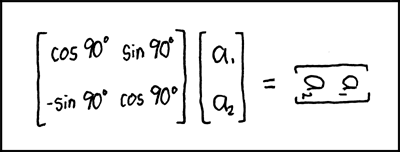
\includegraphics[width=0.3\linewidth]{images/xkcd.png}
	\caption{Source: ``Matrix Transform", xkcd}
\end{figure}

Is there a simpler way to do this?

\clearpage

We note that the sum of each column in the matrix is $10$. Therefore, we think to sum up the equations: \begin{eqnarray*} 10a+10b+10c&=&11+18+21=50 \\ \implies \color{ForestGreen} a+b+c&\color{ForestGreen} =&\color{ForestGreen} 5. \end{eqnarray*} We now eliminate to solve for the variables $b$ and $c$. Subtracting the above relation from the second equation gives \begin{eqnarray*} \left(a+4b+6c\right)-\left(a+b+c\right)&=&18-5=13 \\ \color{blue} 3b+5c &\color{blue}=& \color{blue} 13.\end{eqnarray*} We also multiply the relation by $2$ to eliminate for $b$ and $c$ in the third equation: \begin{eqnarray*} \left(2a+2b+2c\right)-\left(2a+b+3c\right) &=& 2\cdot 5-21=-11 \\ \color{blue} b-c &\color{blue}=&\color{blue} -11. \end{eqnarray*}

We multiply the second equation by $5$ and add: \begin{eqnarray*} \left(3b+5c\right)+\left(5b-5c\right)&=&13-5\cdot 11=-42 \\ 8b &=& -42. \end{eqnarray*}  Therefore, $\displaystyle b=\frac{-42}{8}=\color{orange} \frac{-21}{4}$. Substituting this into $b-c=-11$ gives $$c=11+b=11-\frac{21}{4}=\color{orange} \frac{23}{4}.$$ Finally, plugging both of these into the third equation gives $$2a=21-b-3c=21+\frac{21}{4}-3\cdot \frac{21}{4}=21-12=9.$$ Hence, $a=\color{orange} \frac92$ and $(a,b,c)=\boxed{(\frac{9}{2}, \frac{-21}{4}, \frac{23}{4})}.$ 

\clearpage

\subsection*{Verifying through Mathematica}

The matrix version of the equation is useful to verify through the computer program, Mathematica.  I use the two lines of code: 

\color{Lavender} m = \{\{7, 5, 1\}, \{1, 4, 6\}, \{2, 1, 3\}\} \\ LinearSolve[m, \{11, 18, 21\}]
\color{black} 

Output: \\ \color{ForestGreen} \{9/2, -(21/4), 23/4\}\color{black}
 
This is the same as what we found above!

\end{proof}

\mybox{0.8\textwidth}{\begin{prob}[2014 Purple Comet] Let $x,y,z$ be positive real numbers satisfying the simultaneous equations \begin{eqnarray*} x(y^2+yz+z^2) &=& 3y+10z \\ y(z^2+zx+x^2) &=& 21z+24x \\ z(x^2+xy+y^2) &=& 7x+28y. \end{eqnarray*}  
Find $xy+yz+zx$.  \end{prob}}
\clearpage

\subsection{2014 Purple Comet}
\begin{proof}[Solution]
We note that the equations on the left hand side are symmetric. We therefore think to \textbf{sum} up the equations. I claim that when we do so, the left hand side becomes $(x+y+z)(xy+xz+yz)$. \color{red} Why? \color{black}

Expand out, group, and colour the $xyz$ terms: \begin{eqnarray*} (x+y+z)(xy+xz+yz)=\color{red}\left(x^2y+ x^2z\right)\color{black}+\color{ForestGreen}\left(y^2x+y^2z\right)\color{black}+\color{blue}\left(z^2y+z^2x\right)\color{black}+3xyz \end{eqnarray*} We distribute and colour the other terms: \begin{eqnarray*} x\left(y^2+yz+z^2\right)&=&\color{ForestGreen}y^2x\color{black}+xyz+\color{blue}z^2x \\ y\left(z^2+zx+x^2\right)&=&\color{blue}z^2y\color{black}+xyz+\color{red}x^2y \\ z\left(x^2+xy+y^2\right)&=&\color{red}x^2z\color{black}+xyz+\color{ForestGreen}y^2z. \end{eqnarray*}

\clearpage

Therefore, by proof by colouring, we have showed that summing up the left hand side gives $(x+y+z)(xy+xz+yz)$. Summing up the right hand side gives $$\left(3y+10z\right)+\left(21z+24x\right)+\left(7x+28y\right)=31\left(x+y+z\right).$$ We equate the two of them, and divide through by $x+y+z$ (since it is positive): $$(x+y+z)(xy+xz+yz)=31(x+y+z)\implies xy+xz+yz=\boxed{31}.$$ 

How did I think of the factorization? The motivation behind it came from the problem statement asking to find $xy+yz+zx$! \end{proof}
\clearpage

\subsection{Two More Tricky Symmetry Problems}
\mybox{0.8\textwidth}{ \begin{prob}[Purple Comet 2012] Let $a,b,$ and $c$ be non-zero real numbers such that $$\frac{ab}{a+b}=3,\: \frac{bc}{b+c}=4,\: \text{and } \frac{ca}{c+a}=5.$$ Compute the value of $\displaystyle \frac{abc}{ab+bc+ca}$. \end{prob}\begin{prob}[HMMT 2013] Let $x$ and $y$ be real numbers with $x>y$. Find $x$ if $$x^2y^2+x^2+y^2+2xy=40 \text{ and }xy+x+y=8.$$ \end{prob}}

\subsection{Purple Comet 2012}
The expressions involving $a,b$ in the centered equation look familiar. Where have I seen them before, though? Since they involve fractions, I think to take the \textbf{reciprocal} of all of the equations: $$\frac{a+b}{ab}=\frac13\:,\:\: \frac{b+c}{bc}=\frac14\:,\:\: \text{and } \frac{c+a}{ca}=\frac15.$$ 
Note that we can simplify each of these expressions! For instance, $\frac{a+b}{ab}=\frac{1}{b}+\frac{1}{a}$. Then, the system of equations becomes $$\color{blue}\frac{1}{b}+\frac{1}{a}=\frac13\:,\:\: \frac{1}{c}+\frac{1}{b}=\frac14\:,\:\: \text{and } \frac{1}{a}+\frac{1}{c}=\frac15.$$ 
\clearpage

We continue by taking the reciprocal of the desired expression, $\frac{abc}{ab+bc+ca}$: $$\frac{ab+bc+ca}{abc}=\frac{1}{c}+\frac{1}{a}+\frac{1}{b}.$$ Aha! We've turned this into something we know how to work with. We sum up the three blue equatinos from the previous slide to get $$2\left(\frac1a+\frac1b+\frac1c\right)=\frac13+\frac14+\frac15=\frac{47}{60}.$$ Therefore, $\displaystyle \frac1a+\frac1b+\frac1c=\frac{47}{120}$. We have to take the reciprocal, however, to get $$\frac{abc}{ab+bc+ca}=\frac{1}{\frac1a+\frac1b+\frac1c}=\boxed{\frac{120}{47}}.$$

\clearpage

\subsection{HMMT 2013}
The first thing which jumps out to me is the weirdness of this system. We have a bunch of terms of degrees $1$ and $2$ throughout. In the second equation, we see that the terms $xy$ and $x+y$ show up a lot. Furthermore, $(x+y)^2=x^2+y^2+2xy$. This motivations the \textit{substitutions}, $a=xy$ and $b=x+y$. The system then becomes: $$a^2+b^2=40\:,\: a+b=8.$$  
We square the second equation to arrive at $(a+b)^2=a^2+2ab+b^2=64$. 

Subtracting this from the first equation gives $2ab=64-40=24\implies ab=12.$

Solving this system, we now see that $\color{blue} (a,b)=(2,6), (6,2)$.
\clearpage

If $(a,b)=(6,2)$, then we have $xy=6$ and $x+y=2$. We use the identity that $$(z-x)(z-y)=z^2-z(x+y)+xy$$ to create a quadratic equation with roots $z=x$ and $z=y$. The quadratic for this case is $z^2-2z+6$. This has \textit{discriminant} $\Delta=2^2-4\cdot 6=-20$, therefore, it does not have positive real solutions.

On the other hand, when $(a,b)=(2,6)$, we have $xy=2$ and $x+y=6$. The quadratic for this case is $z^2-6z+2$. Completing the square, we can solve the quadratic: $$z^2-6z+2=(z-3)^2-7\implies z=3\pm \sqrt{7}.$$ Since $x>y$, we have $x=\boxed{3+\sqrt{7}}$.  



\section{Weird Functions}

\mybox{0.8\textwidth}{\begin{prob}[2000 AMC 12]  Let $f$ be a function for which $f(x/3) = x^2 + x + 1$. Find the sum of all values of $z$ for which $f(3z) = 7$. \end{prob} \begin{prob}[Mandelbrot] Let $f$ be a function such that when $a+b=2^n$ for $a,b,n$ integers, then $f(a)+f(b)=n^2$. What is $f(2002)$? \end{prob} \begin{prob}[Mandelbrot] Let $f$ be a function which takes $2$ inputs as arguments.The value of $f$ is defined recursively: $f(x,y)=x+f(x-1, x-y)$. If $f(1,0)=5$, find $f(5,2)$. \end{prob}}

\subsection{2000 AMC 12}
The function that we are given is somewhat strange. It takes as input $x/3$ and returns a value based upon this. We can modify the input, however, by setting \color{blue} $x=9y$ \color{black} for real $y$. Plugging this into the definition of the function gives $$f(3y)=(9y)^2+9y+1.$$ We want the sum of the values $z$ for which \begin{eqnarray*} f(3z)=(9z)^2+9y+1&=&7 \\ 81z^2+9z-6 &=& 0. \end{eqnarray*}

If the roots of this quadratic are $r_1$ and $r_2$, then, we can rewrite with leading coefficient $81$ as: $$f(3z)=81(z-r_1)(z-r_2)=81z^2+9z-6.$$ Equating the $z$ coefficient gives $$81(-r_1-r_2)=9\implies r_1+r_2=\boxed{\frac{-1}{9}}.$$ 

If you knew Vieta's formula, we could use the fact that the sum of the roots is $\displaystyle -\frac{b}{a}=-\frac{1}{9}$. If you don't know Vieta's formula, don't worry! We'll cover it shortly.  

\clearpage

\subsection{2002 Mandelbrot}

The condition we're given again is odd. 

\section{Sequences and Series}
\mybox{0.95\textwidth}{\begin{prob}[2003 AMC 10] The first four terms in an arithmetic sequence are $x+y, x-y, xy$, and $\frac{x}{y}$, in that order. What is the fifth term? \end{prob} \begin{prob}[USAMTS] In an attempt to copy down a sequence of six positive integers in arithmetic progression, a student wrote down the five numbers $113, 137, 149, 155, 173$, accidentally omitting one. He later discovered that he also miscopied one of them. Can you help him recover the original sequence? \end{prob}}

\clearpage \mybox{0.8\textwidth}{\begin{prob}[1986 AIME] The pages of a book are numbered $1_{}^{}$ through $n_{}^{}$. When the page numbers of the book were added, one of the page numbers was mistakenly added twice, resulting in an incorrect sum of $1986_{}^{}$. What was the number of the page that was added twice? \end{prob}\begin{prob}[1994 AHSME] Suppose $x,y,z$ is a geometric sequence with common ratio $r$ and $x \neq y$. If $x, 2y, 3z$ is an arithmetic sequence, then find the value of $r$. \end{prob}}





\end{document}  